\documentclass{article}
\usepackage{leonine,amsmath,amssymb,amsthm,graphicx,setspace}%%xy, setspace, amscd (commutative diagram)
\title{Notes}
\author{Eric Purdy \footnote{Department of Computer Science, University of Chicago. Email: epurdy@uchicago.edu}}

%%\doublespace

\begin{document}
\maketitle

\setcounter{section}{0}

\section{Assembling Datasets} 

\section{Grammatical Shape Models}

\subsection{A hand-built grammar}

Here we are drawing a grammar. We have built this grammar by hand, by
taking the following curve, and specifying a decomposition of it:

\includegraphics[width=2in]{./1.grammars/hand_built/hand_built_curve.eps}

Here is the grammar:

Here are some samples from the grammar:

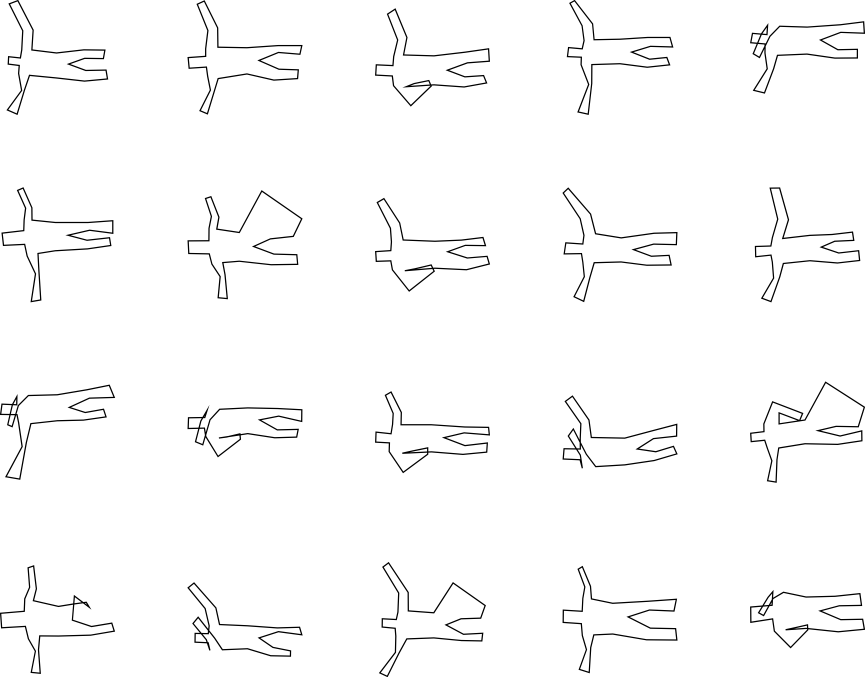
\includegraphics[width=6in]{output/3.learning/incremental/gram.19.d/samples.png}



\section{Parsing}


\subsection{One-to-one}

Here we have two curves given by hand-annotation of the Romer
dataset. We build a grammar from the curve on the left, using a
hand-built set of constituents. We then parse the curve on the right,
and show the Viterbi parse by showing the correspondences between the
two curves.

Because there are no missing or extra points, this is straightforward.

%% we can use \input{} here to incorporate dynamically generated text

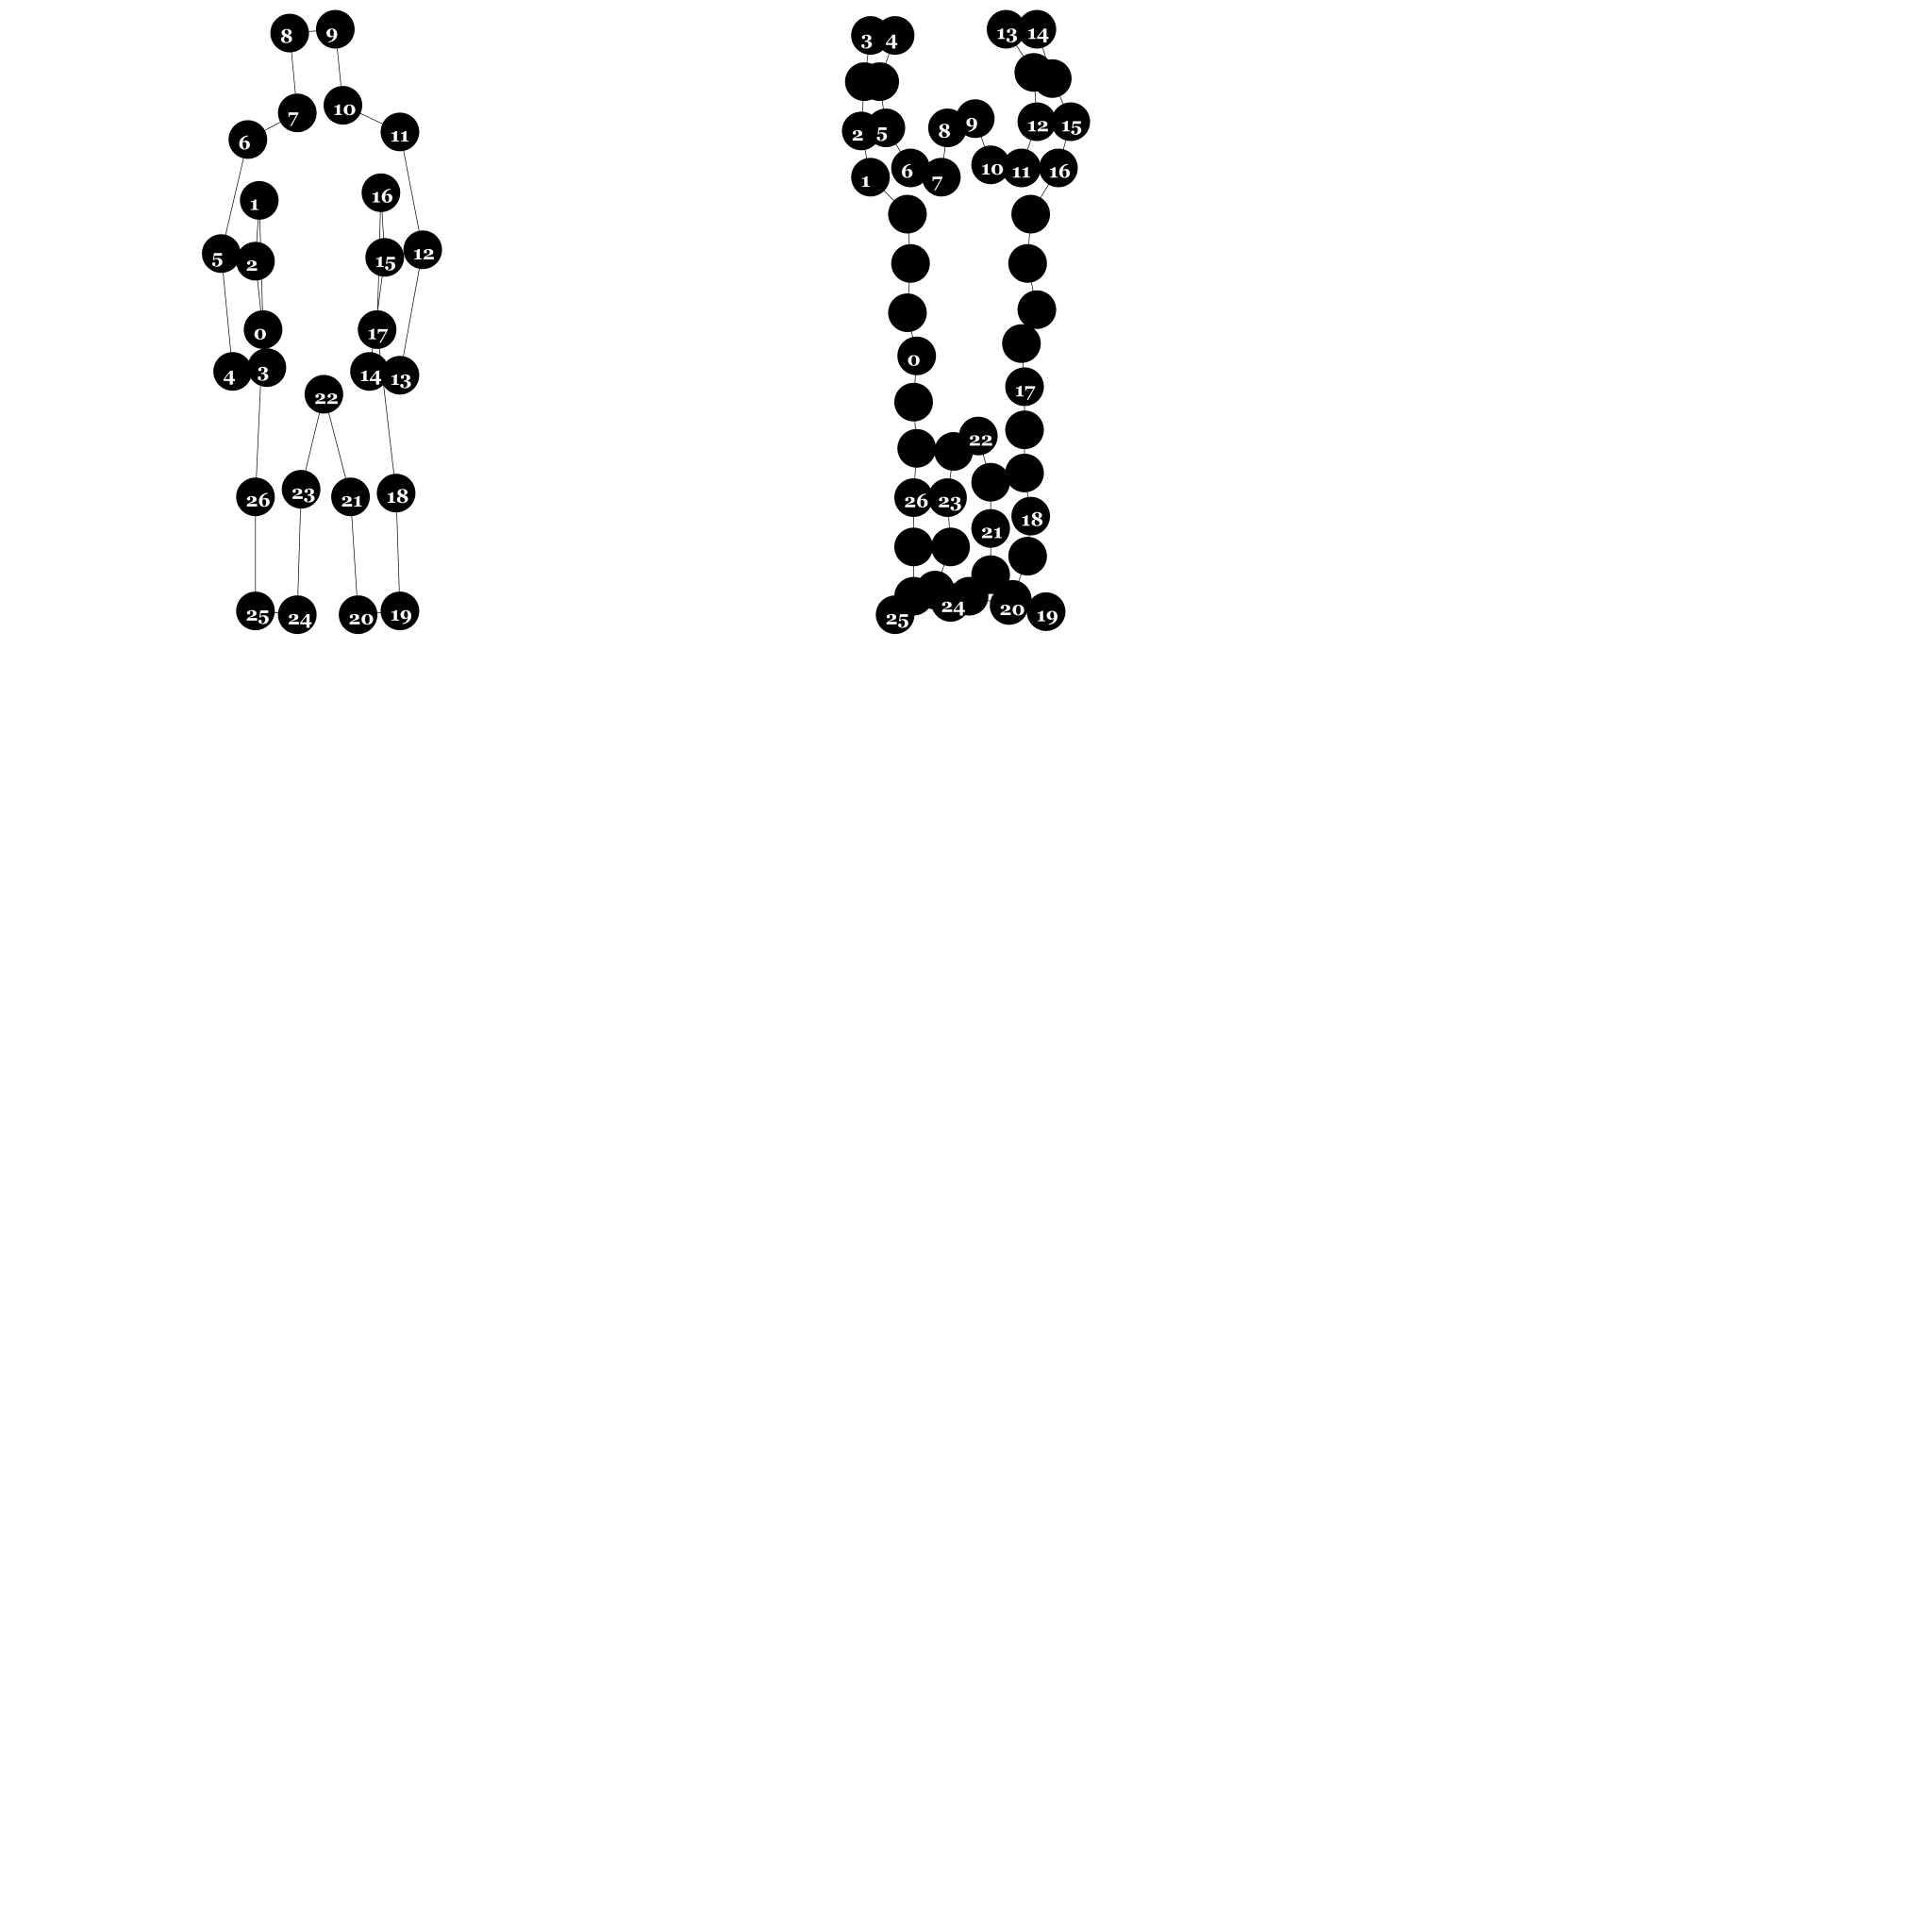
\includegraphics[width=6in]{./2.parsing/one_to_one/parse.eps}



\section{EM}

\subsection{Simple tuning}

Here is our example curve, from which we build a grammar with hand-chosen rules.

\includegraphics[width=2in]{./3.em/simple_tuning/examples.eps}

Here are our training curves:

\includegraphics[width=2in]{./3.em/simple_tuning/training.eps}

Here is the grammar:

\subsubsection{Initial}
Here are some samples from the grammar:

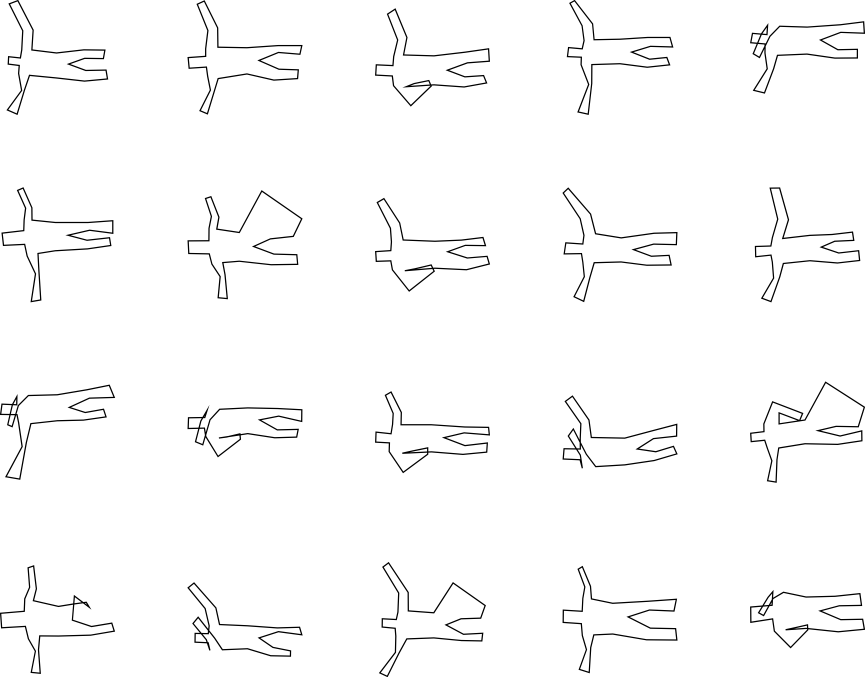
\includegraphics[width=6in]{output/3.learning/incremental/gram.19.d/samples.png}



\subsubsection{Round 1}
Here are some samples from the grammar:

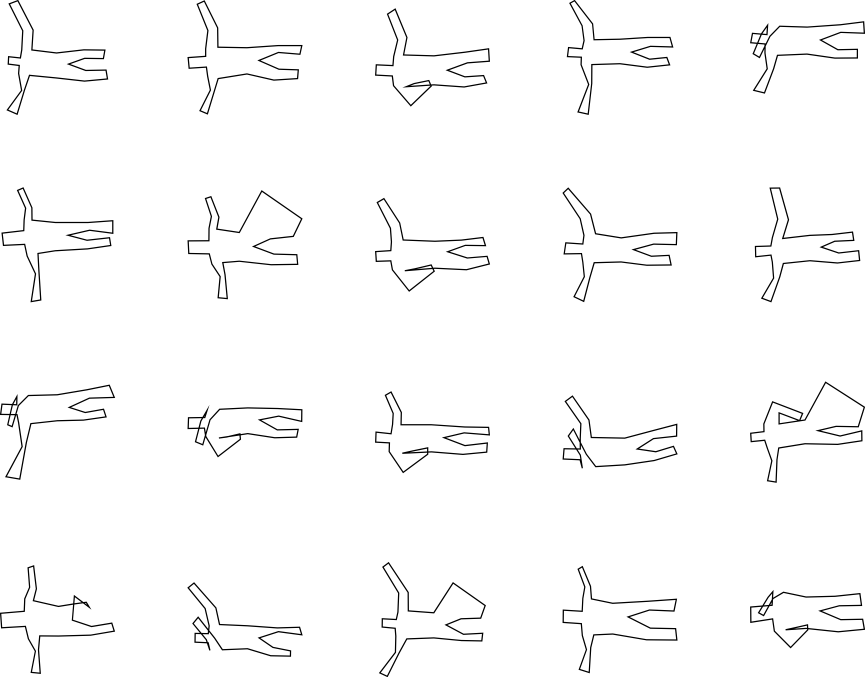
\includegraphics[width=6in]{output/3.learning/incremental/gram.19.d/samples.png}


\subsubsection{Round 2}
Here are some samples from the grammar:

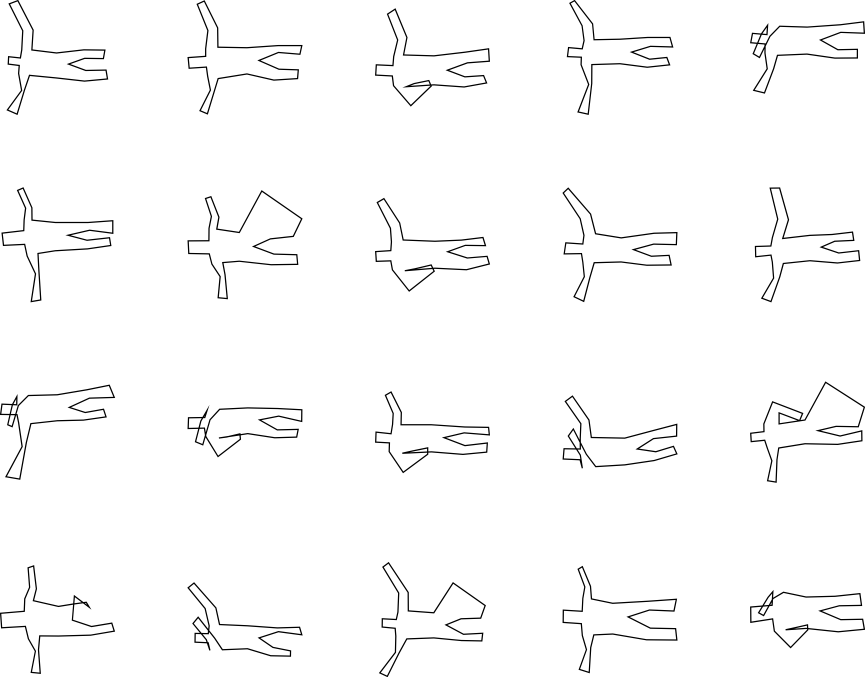
\includegraphics[width=6in]{output/3.learning/incremental/gram.19.d/samples.png}


\subsubsection{Round 3}
Here are some samples from the grammar:

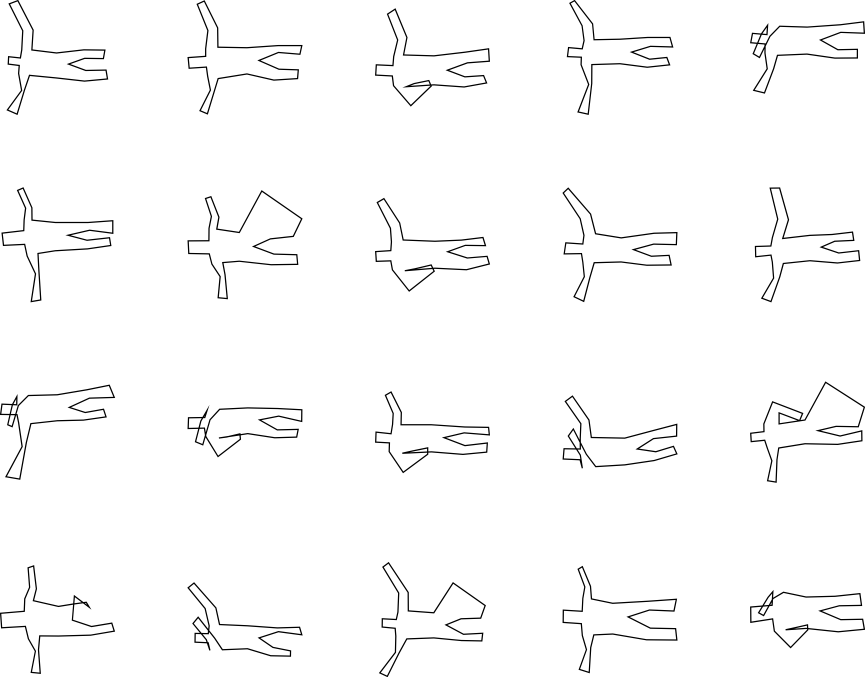
\includegraphics[width=6in]{output/3.learning/incremental/gram.19.d/samples.png}


\subsubsection{Round 4}
Here are some samples from the grammar:

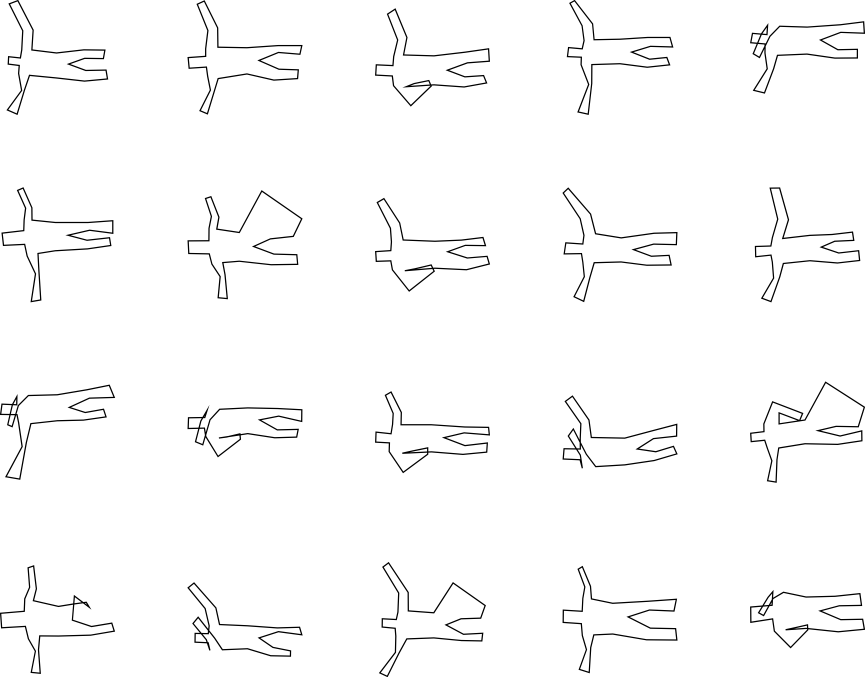
\includegraphics[width=6in]{output/3.learning/incremental/gram.19.d/samples.png}


\subsubsection{Round 5}
Here are some samples from the grammar:

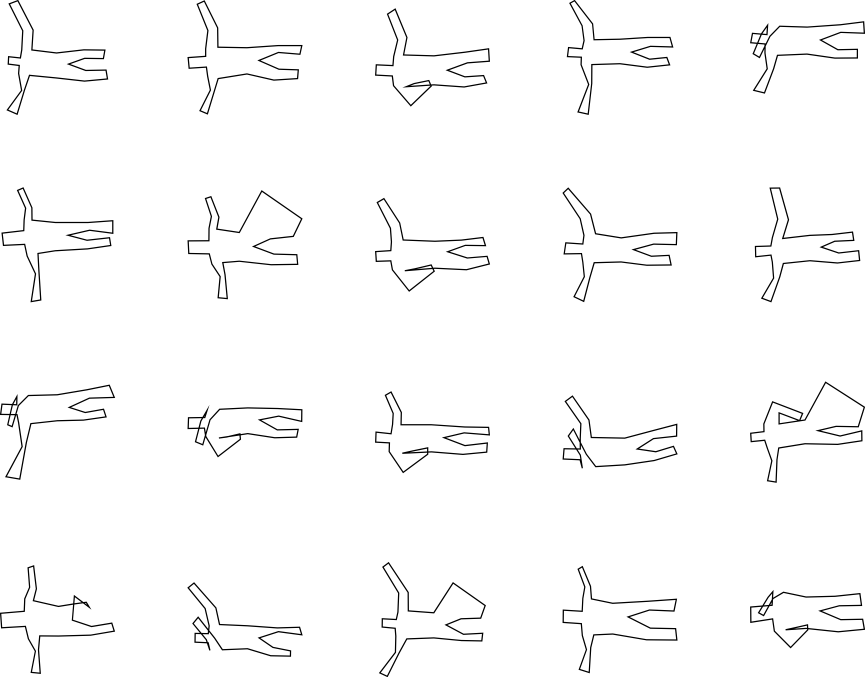
\includegraphics[width=6in]{output/3.learning/incremental/gram.19.d/samples.png}




\section{Parsing in Cluttered Images}

\section{Using SDF's in Other Domains}

\section{Learning Structure}
\documentclass{article}
\usepackage{leonine,amsmath,amssymb,amsthm,graphicx}%%xy, setspace, amscd (commutative diagram)
\title{Notes}
\author{Eric Purdy \footnote{Department of Computer Science, University of Chicago. Email: epurdy@uchicago.edu}}

%%\doublespace

\begin{document}
\maketitle

In Bronstein Bronstein Bruckstein Kimmel (Analysis of 2-D Non-rigid
shapes), there is a list of approaches to shape segmentation:

\bitem
\item Convex or near-convex subsets 
\bitem
\item Hoffman and Richards 1984
\item Koenderink and van Doorn 1981
\eitem
\item Primitive geometric objects
\bitem
\item Binford 1987
\item Biderman 1985
\item Bajcsy and Solina 1987
\item Pentland 1987
\eitem
\item Parametric description derived from a model of the shape class
\bitem
\item Brooks 1981
\item Helo-Or and Werman 1994
\eitem
\eitem

\section{other stuff}

Mark Johnson on EM vs. gibbs vs. variational bayes
http://nlpers.blogspot.com/2007/07/collapsed-gibbs.html

Variational Bayes
http://en.wikipedia.org/wiki/Variational_Bayesian_methods
http://en.wikipedia.org/wiki/Variational_message_passing
http://en.wikipedia.org/wiki/Expectation-maximization#Relation_to_variational_Bayes_methods

wikipedia had link to original EM paper considered bayesian
Laird and other people?

wikipedia

naacl 2007 mark johnson gives good alpha

random HOSVD paper linked from wikipedia

other stuff related to KL in other notes



\end{document}


\section{Learning Texture}

\begin{figure}
\includegraphics[width=0.45\linewidth]{experiments/7.texture/scaled_nts/output.d/scaled_nts_training_1.png}
\hfill
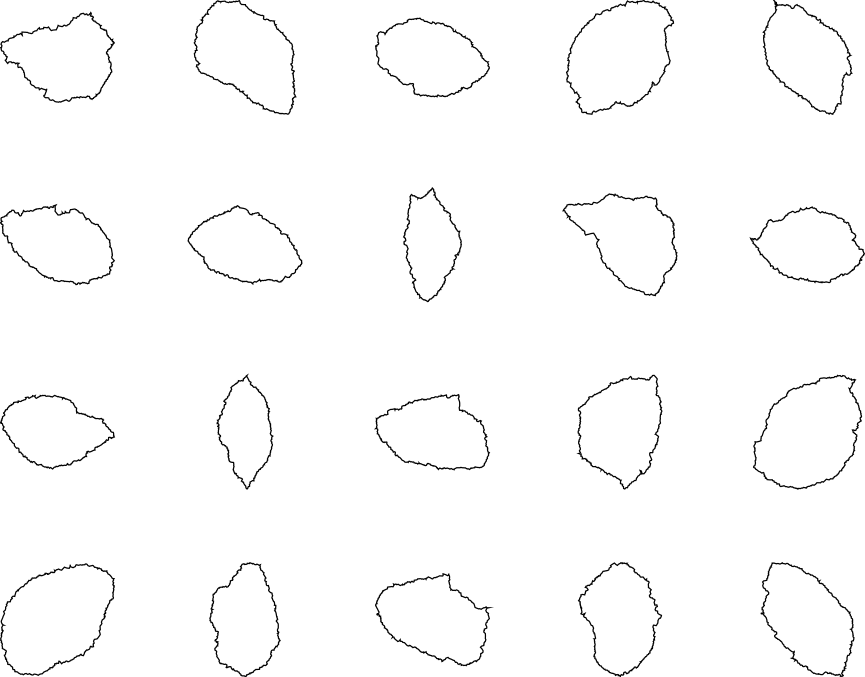
\includegraphics[width=0.45\linewidth]{experiments/7.texture/scaled_nts/output.d/scaled_nts_1.png}
\\\vspace{3\baselineskip}
\includegraphics[width=0.45\linewidth]{experiments/7.texture/scaled_nts/output.d/scaled_nts_training_2.png}
\hfill
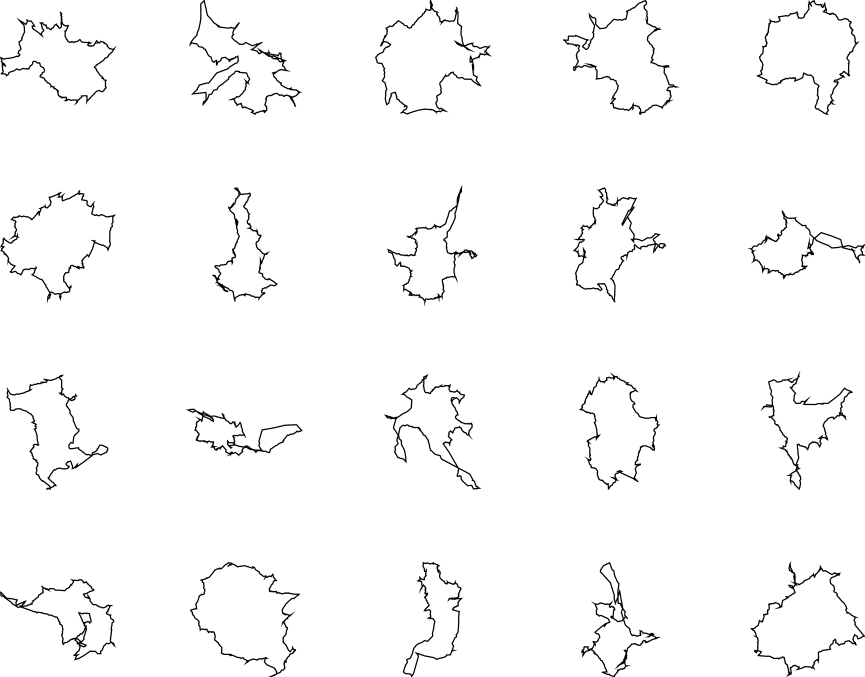
\includegraphics[width=0.45\linewidth]{experiments/7.texture/scaled_nts/output.d/scaled_nts_2.png}
\\\vspace{3\baselineskip}
\includegraphics[width=0.45\linewidth]{experiments/7.texture/scaled_nts/output.d/scaled_nts_training_3.png}
\hfill
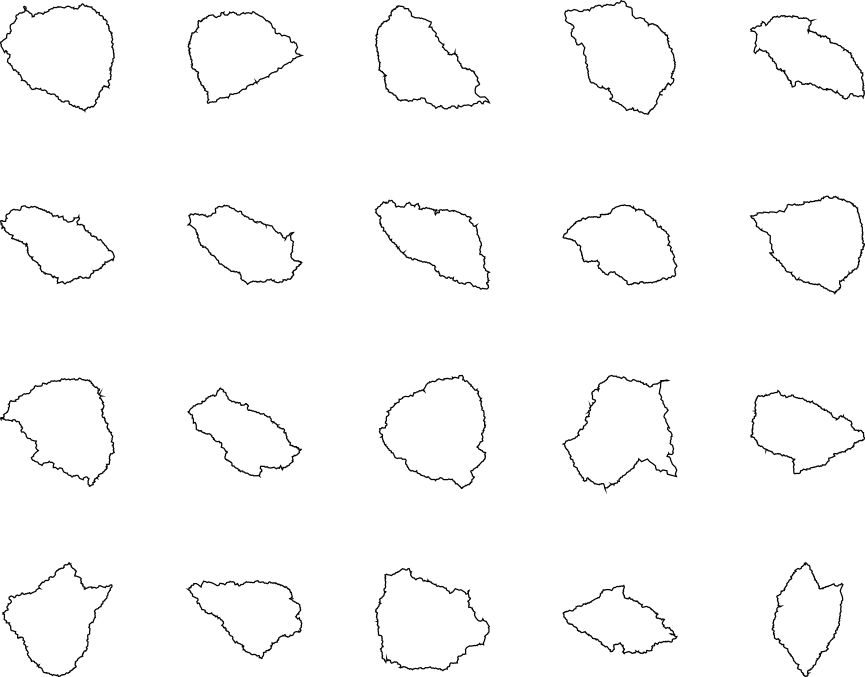
\includegraphics[width=0.45\linewidth]{experiments/7.texture/scaled_nts/output.d/scaled_nts_3.png}
\\\vspace{3\baselineskip}
\includegraphics[width=0.45\linewidth]{experiments/7.texture/scaled_nts/output.d/scaled_nts_training_4.png}
\hfill
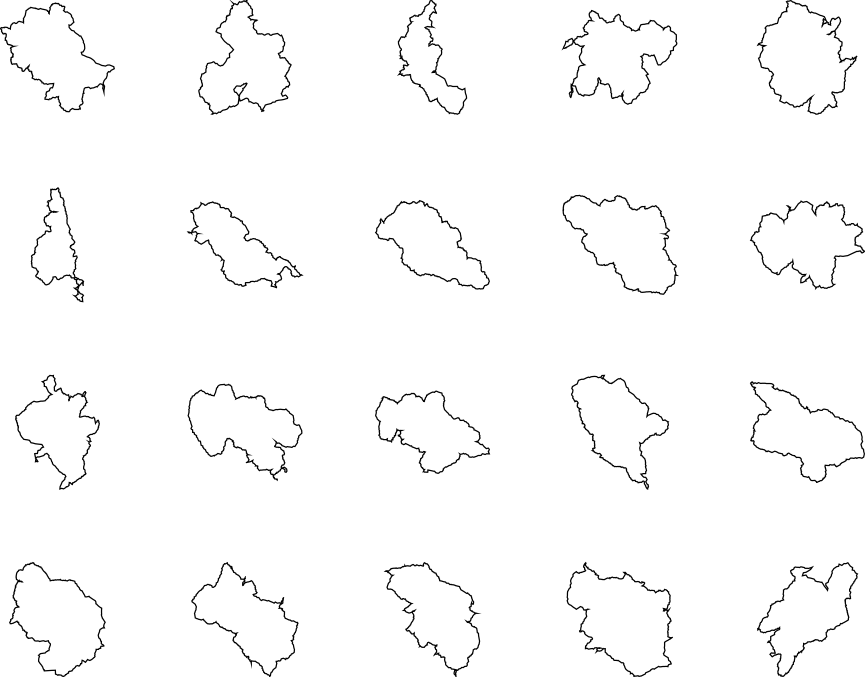
\includegraphics[width=0.45\linewidth]{experiments/7.texture/scaled_nts/output.d/scaled_nts_4.png}
\\\vspace{3\baselineskip}
\includegraphics[width=0.45\linewidth]{experiments/7.texture/scaled_nts/output.d/scaled_nts_training_5.png}
\hfill
\includegraphics[width=0.45\linewidth]{experiments/7.texture/scaled_nts/output.d/scaled_nts_5.png}
\caption{Training on left, samples on right.}
\end{figure}

\begin{figure}
\includegraphics[width=0.45\linewidth]{experiments/7.texture/scaled_nts/output.d/scaled_nts_training_6.png}
\hfill
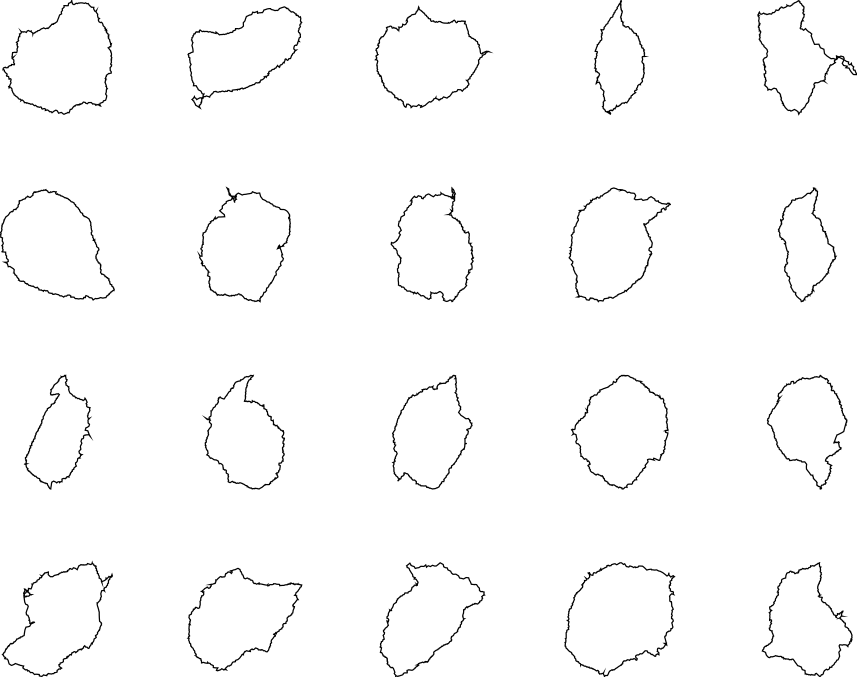
\includegraphics[width=0.45\linewidth]{experiments/7.texture/scaled_nts/output.d/scaled_nts_6.png}
\\\vspace{3\baselineskip}
\includegraphics[width=0.45\linewidth]{experiments/7.texture/scaled_nts/output.d/scaled_nts_training_7.png}
\hfill
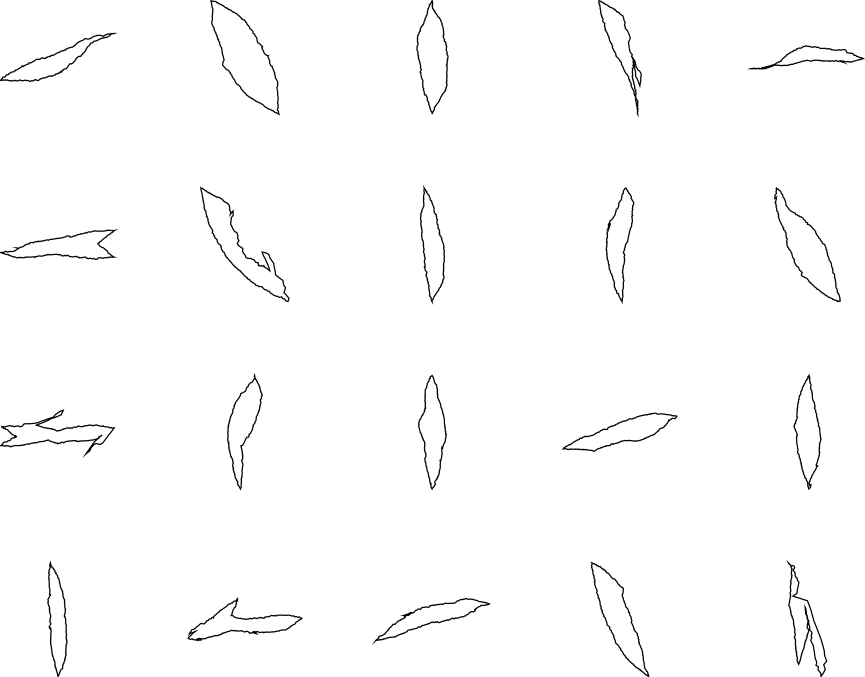
\includegraphics[width=0.45\linewidth]{experiments/7.texture/scaled_nts/output.d/scaled_nts_7.png}
\\\vspace{3\baselineskip}
\includegraphics[width=0.45\linewidth]{experiments/7.texture/scaled_nts/output.d/scaled_nts_training_8.png}
\hfill
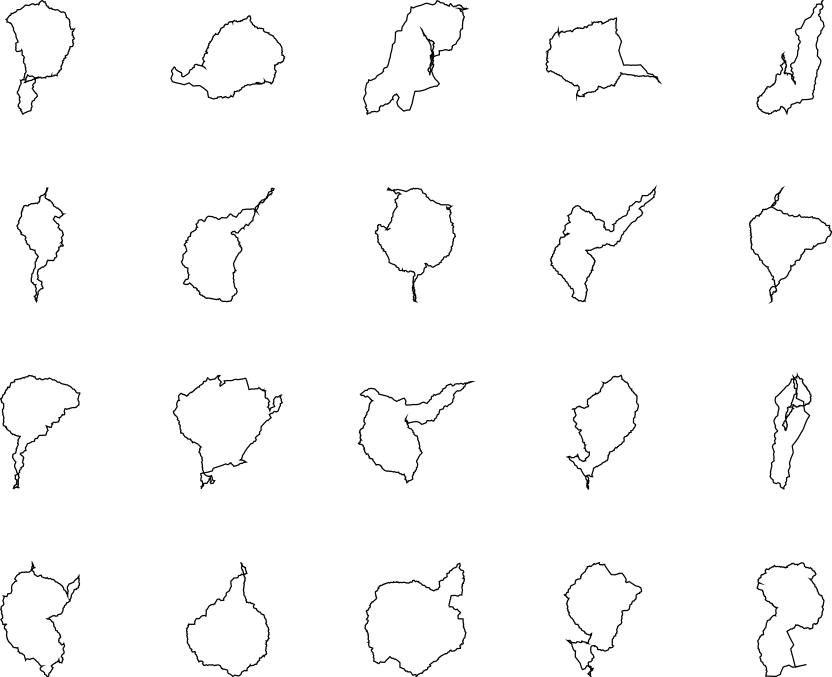
\includegraphics[width=0.45\linewidth]{experiments/7.texture/scaled_nts/output.d/scaled_nts_8.png}
\\\vspace{3\baselineskip}
\includegraphics[width=0.45\linewidth]{experiments/7.texture/scaled_nts/output.d/scaled_nts_training_9.png}
\hfill
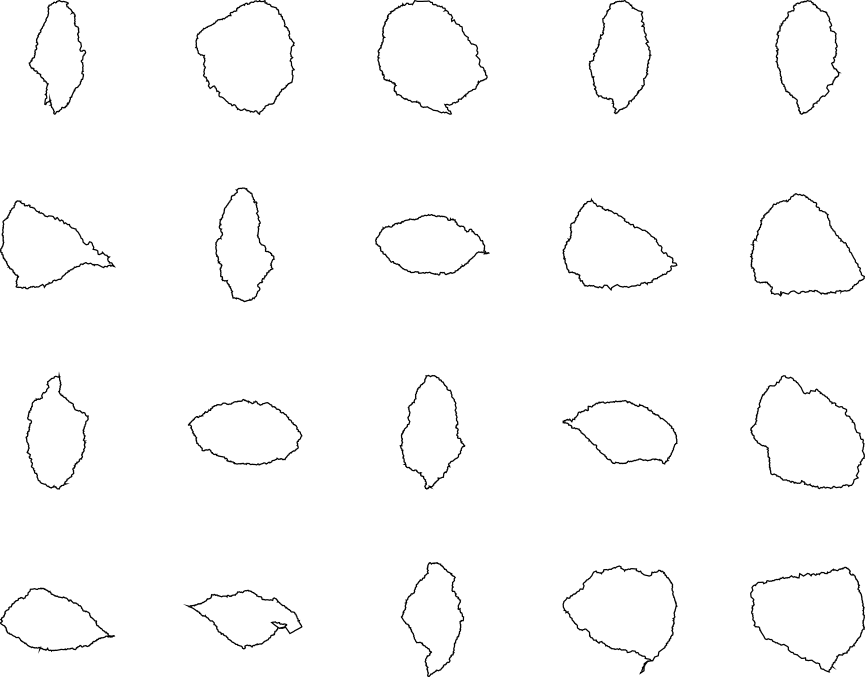
\includegraphics[width=0.45\linewidth]{experiments/7.texture/scaled_nts/output.d/scaled_nts_9.png}
\\\vspace{3\baselineskip}
\includegraphics[width=0.45\linewidth]{experiments/7.texture/scaled_nts/output.d/scaled_nts_training_10.png}
\hfill
\includegraphics[width=0.45\linewidth]{experiments/7.texture/scaled_nts/output.d/scaled_nts_10.png}
\caption{Training on left, samples on right.}
\end{figure}

\begin{figure}
\includegraphics[width=0.45\linewidth]{experiments/7.texture/scaled_nts/output.d/scaled_nts_training_11.png}
\hfill
\includegraphics[width=0.45\linewidth]{experiments/7.texture/scaled_nts/output.d/scaled_nts_11.png}
\\\vspace{3\baselineskip}
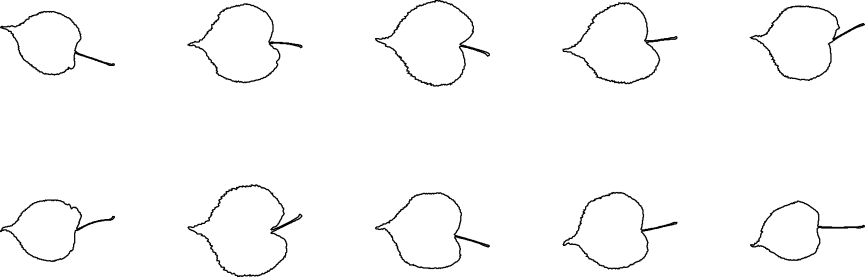
\includegraphics[width=0.45\linewidth]{experiments/7.texture/scaled_nts/output.d/scaled_nts_training_12.png}
\hfill
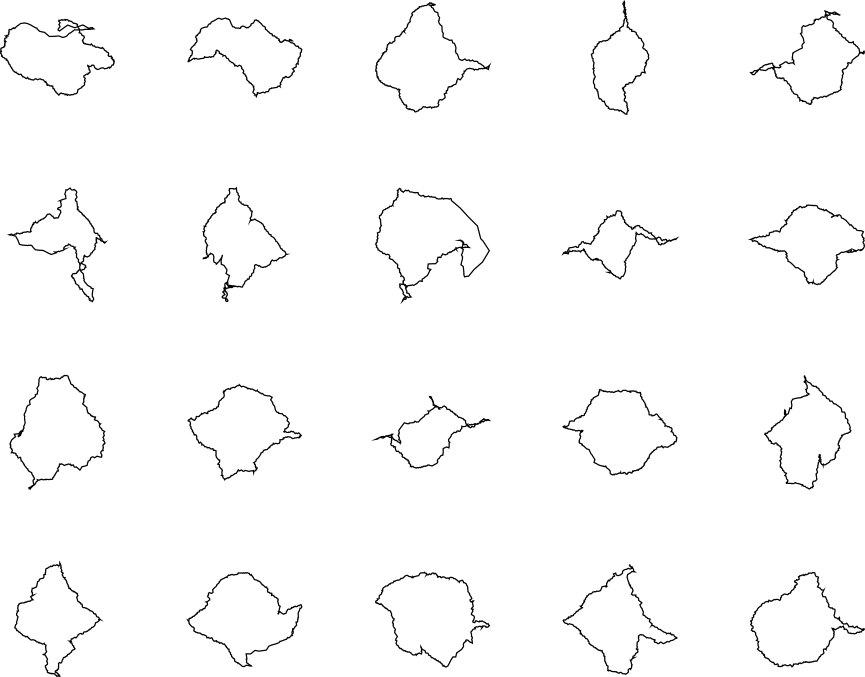
\includegraphics[width=0.45\linewidth]{experiments/7.texture/scaled_nts/output.d/scaled_nts_12.png}
\\\vspace{3\baselineskip}
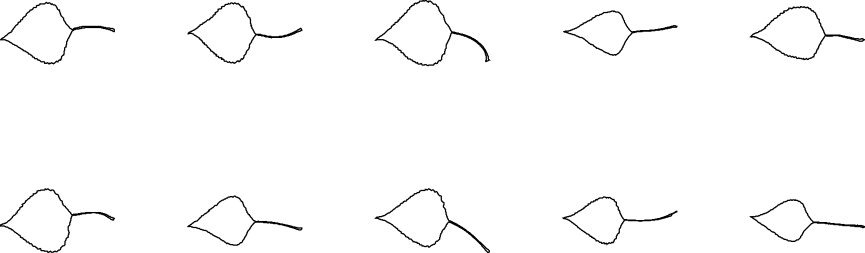
\includegraphics[width=0.45\linewidth]{experiments/7.texture/scaled_nts/output.d/scaled_nts_training_13.png}
\hfill
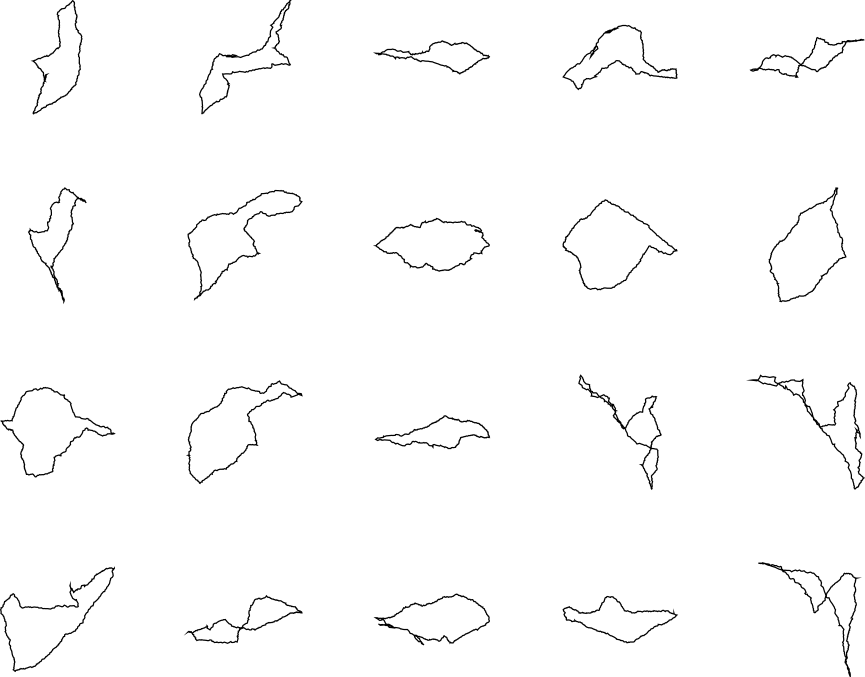
\includegraphics[width=0.45\linewidth]{experiments/7.texture/scaled_nts/output.d/scaled_nts_13.png}
\\\vspace{3\baselineskip}
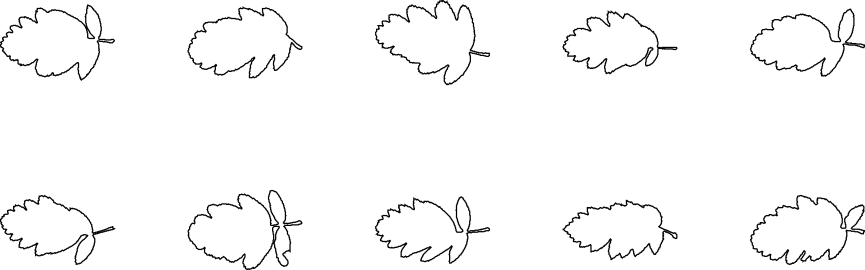
\includegraphics[width=0.45\linewidth]{experiments/7.texture/scaled_nts/output.d/scaled_nts_training_14.png}
\hfill
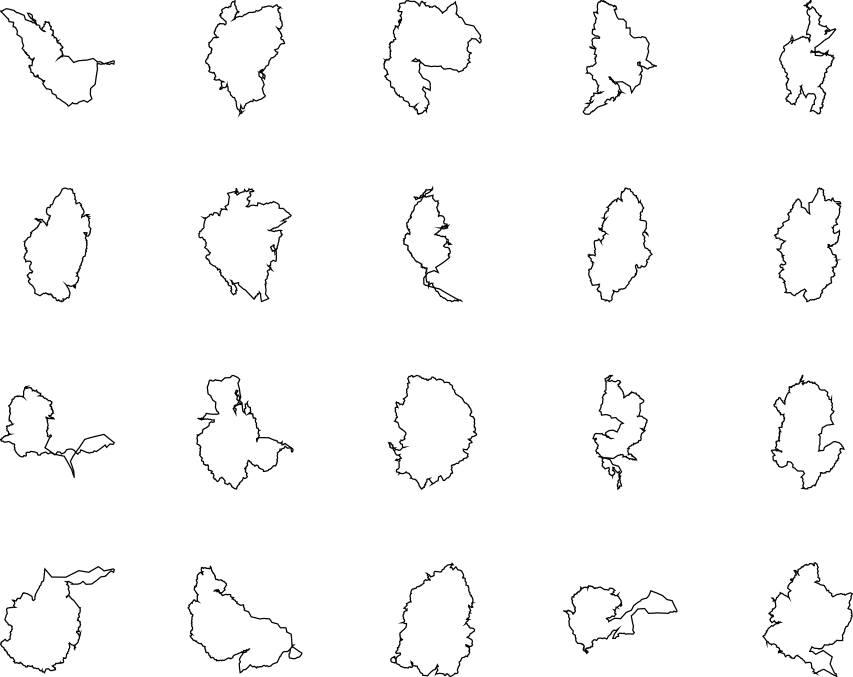
\includegraphics[width=0.45\linewidth]{experiments/7.texture/scaled_nts/output.d/scaled_nts_14.png}
\\\vspace{3\baselineskip}
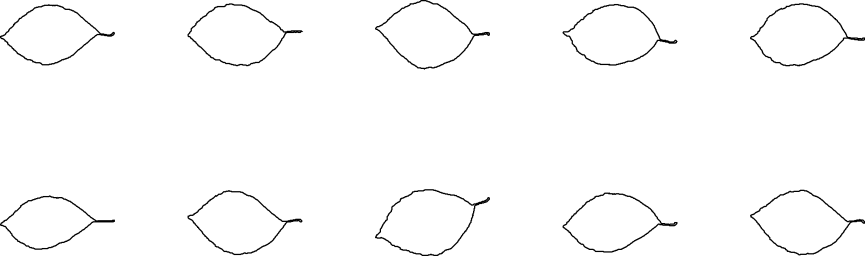
\includegraphics[width=0.45\linewidth]{experiments/7.texture/scaled_nts/output.d/scaled_nts_training_15.png}
\hfill
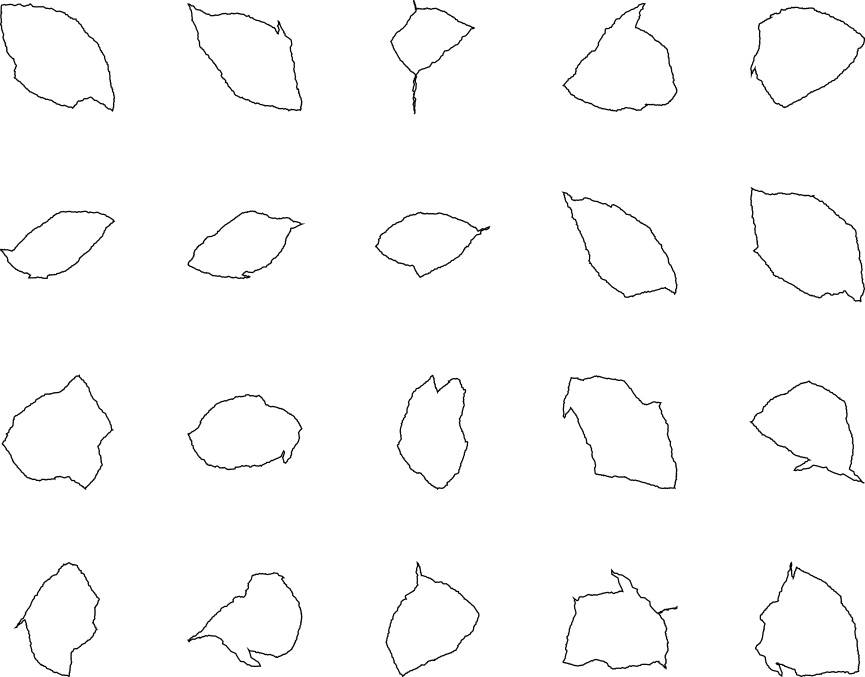
\includegraphics[width=0.45\linewidth]{experiments/7.texture/scaled_nts/output.d/scaled_nts_15.png}
\caption{Training on left, samples on right.}
\end{figure}


\end{document}